\documentclass[12pt]{article}

\usepackage{sbc-template}
\usepackage{graphicx}
\usepackage{url}
\usepackage{hyphenat}
\usepackage[utf8]{inputenc}
\usepackage[brazil]{babel}

% Configurações para evitar quebras de margem com links longos
\sloppy

\title{Farol: IAssistente Intergeracional (Tutoria Reversa) \\ Mediação Tecnológica Inteligente e Acessibilidade Cognitiva para Inclusão Digital de Idosos e PcD}

\author{Asafe Almeida Tork$^1$, José Ruan Costa Ferreira$^1$, \\ Renan Rondinelli da Silva$^1$, Claudia Emanuele Monteiro Reis$^1$, \\ Paulo Gustavo da Silva Gomes$^1$, José Gustavo da Silva Ribeiro$^1$, \\ Marcos Vinicios$^1$, Jefenson Dultra$^1$}

\address{Instituto Federal do Pará (IFPA) \\
  Campus Bragança \\
  68600-000 -- Bragança -- PA -- Brasil \\
  \email{asafetork@gmail.com, orientador@ifpa.edu.br, marcus.brito@ifpa.edu.br}
}

\begin{document}

\maketitle

\begin{abstract}
  The contemporary scenario of digital transformation imposes an interaction dynamic mediated by complex interfaces, which frequently neglect the cognitive and generational diversity of citizens. Elderly people and people with disabilities (PwD) face severe barriers to interpreting essential portals, such as Gov.br. Although accessibility guidelines such as the Web Content Accessibility Guidelines (WCAG 2.1) exist, their implementation in Brazil mostly serves static screen readers, failing in the fundamental pillar of comprehensibility. This work presents the proposal of the IAssistente Intergeracional (Projeto Farol), an open-source platform based on the concept of reverse tutoring. Adapted for feasible execution in High School by low-income students, the solution uses accessible language models and local processing to simplify web navigation without generating paid API costs or advanced hardware requirements.
\end{abstract}

\begin{resumo}
  O cenário contemporâneo da transformação digital impõe uma dinâmica de interação mediada por interfaces complexas, as quais frequentemente negligenciam a diversidade cognitiva e geracional dos cidadãos. Idosos e pessoas com deficiência (PcD) enfrentam severas barreiras para interpretar portais essenciais, como o Gov.br. Embora existam diretrizes de acessibilidade como a WCAG 2.1, sua implementação no Brasil atende predominantemente a leitores de tela estáticos, falhando na compreensibilidade. Este trabalho apresenta a proposta do IAssistente Intergeracional (Projeto Farol), uma plataforma de código aberto baseada em tutoria reversa. Adaptada para execução viável no Ensino Médio por alunos de baixa renda, a solução utiliza modelos de linguagem acessíveis e processamento local para simplificar a navegação web sem gerar custos de APIs pagas ou exigências de hardware avançado.
\end{resumo}

\section{Introdução}

O avanço acelerado da digitalização de serviços públicos no Brasil, centralizado em plataformas como o Gov.br, tornou o acesso a sistemas web um requisito fundamental para o exercício da cidadania. No entanto, a complexidade visual e a densidade de informações dessas interfaces criam barreiras cognitivas significativas, especialmente para a terceira idade e pessoas neurodivergentes. Essas barreiras frequentemente privam os usuários de sua autonomia, exigindo o auxílio presencial constante de terceiros para tarefas básicas, como consultas médicas ou validações de cadastros sociais.

Apesar das recomendações internacionais de acessibilidade, como a \emph{Web Content Accessibility Guidelines} (WCAG 2.1) \cite{w3c_wcag21}, a maioria dos sites governamentais limita-se a ajustes estruturais básicos para leitores de tela estáticos, ignorando aspectos de clareza conceitual e facilidade de navegação \cite{wcge_govbr}.

Diante dessa problemática, o Projeto Farol (IAssistente Intergeracional) propõe uma solução baseada em tutoria reversa: em vez de realizar a tarefa pelo usuário, o assistente guia-o passo a passo através de destaques visuais simples e orientação por voz nativa. O projeto foi reestruturado tecnologicamente para permitir que alunos do 2º ano do Ensino Médio de escolas públicas desenvolvam a aplicação utilizando ferramentas gratuitas e eficientes.

\section{Trabalhos Relacionados}

A literatura recente em Interação Humano-Computador (IHC) aponta caminhos para mitigar a exclusão digital. Barros et al. identificaram falhas estruturais em portais públicos por auditoria automatizada \cite{wcge_govbr}, porém focaram apenas no diagnóstico passivo. O Projeto Farol diferencia-se ao atuar ativamente em tempo real sobre a interface.

Silva et al. demonstraram o uso de Modelos de Linguagem de Larga Escala (LLMs) para a simplificação textual voltada a estudantes neurodivergentes \cite{ctrle_2025}. A presente proposta amplia esse conceito para o contexto utilitário e cidadão de adultos e idosos. Ademais, programas tradicionais de letramento digital \cite{wics_2022} possuem limitações de escala e riscos de privacidade humana. O Farol resolve isso automatizando a mediação com privacidade garantida no próprio dispositivo móvel.

\section*{Análise de Viabilidade Técnica e Econômica (Ensino Médio / Baixa Renda)}

Para garantir que o projeto seja totalmente viável para alunos do 2º ano do Ensino Médio do IFPA, foram realizadas adaptações essenciais:

\begin{itemize}
  \item \textbf{Custo Zero de Infraestrutura:} substituição de APIs pagas por modelos \emph{open source} executados em servidores gratuitos (Hugging Face / Render / Supabase) e plano gratuito do Google Gemini API.
  \item \textbf{Compatibilidade com Celulares Populares:} substituição do motor GeckoView pelo Android WebView nativo, reduzindo o tamanho do aplicativo de \textasciitilde 80~MB para $<$10~MB e garantindo execução fluida em \emph{smartphones} de entrada.
  \item \textbf{Autonomia Offline:} uso da síntese de voz nativa do Android (TTS) e armazenamento de roteiros de navegação (``\emph{skills}'') via banco SQLite/Preferences local, economizando dados móveis (3G/4G).
\end{itemize}

\section{Metodologia e Arquitetura do Sistema}

O sistema é estruturado em uma arquitetura leve, otimizada para o ecossistema Android padrão, conforme o resumo das adaptações por módulo na Tabela~\ref{tab:viabilidade}.

\begin{table}[!ht]
  \centering
  \caption{Adaptação de viabilidade técnica e econômica por módulo do sistema.}
  \label{tab:viabilidade}
  \begin{tabular}{|p{3.0cm}|p{4.6cm}|p{5.8cm}|}
    \hline
    \textbf{Módulo} & \textbf{Especificação Original} & \textbf{Adaptação de Viabilidade (Versão Atual)} \\ \hline
    Interface / Captura & GeckoView (alta carga, APK grande) & Android WebView nativo + \emph{scripts} de injeção leve de acessibilidade (DOM). \\ \hline
    Privacidade Local & Filtro determinístico de dados & Sanitizador em JS local: remove senhas e CPFs antes do envio de dados à rede. \\ \hline
    Inteligência / LLM & APIs pagas por uso (\emph{tokens} em \$) & Gemini API (tier gratuito) ou modelos locais (Phi-3 / Llama 3 via \emph{backend} gratuito). \\ \hline
    Síntese de Voz & Serviços de voz em nuvem & Android Text-to-Speech (TTS) nativo: operação 100\% \emph{offline} e sem custos. \\ \hline
  \end{tabular}
\end{table}

A Figura~\ref{fig:fluxo} apresenta o fluxo de interação do Farol: a página aberta no navegador integrado (Android WebView) é capturada por meio da árvore de acessibilidade, o roteiro de navegação é simplificado pelo modelo de linguagem e devolvido ao usuário como orientação por voz acompanhada de destaque visual passo a passo.

\begin{figure}[!ht]
  \centering
  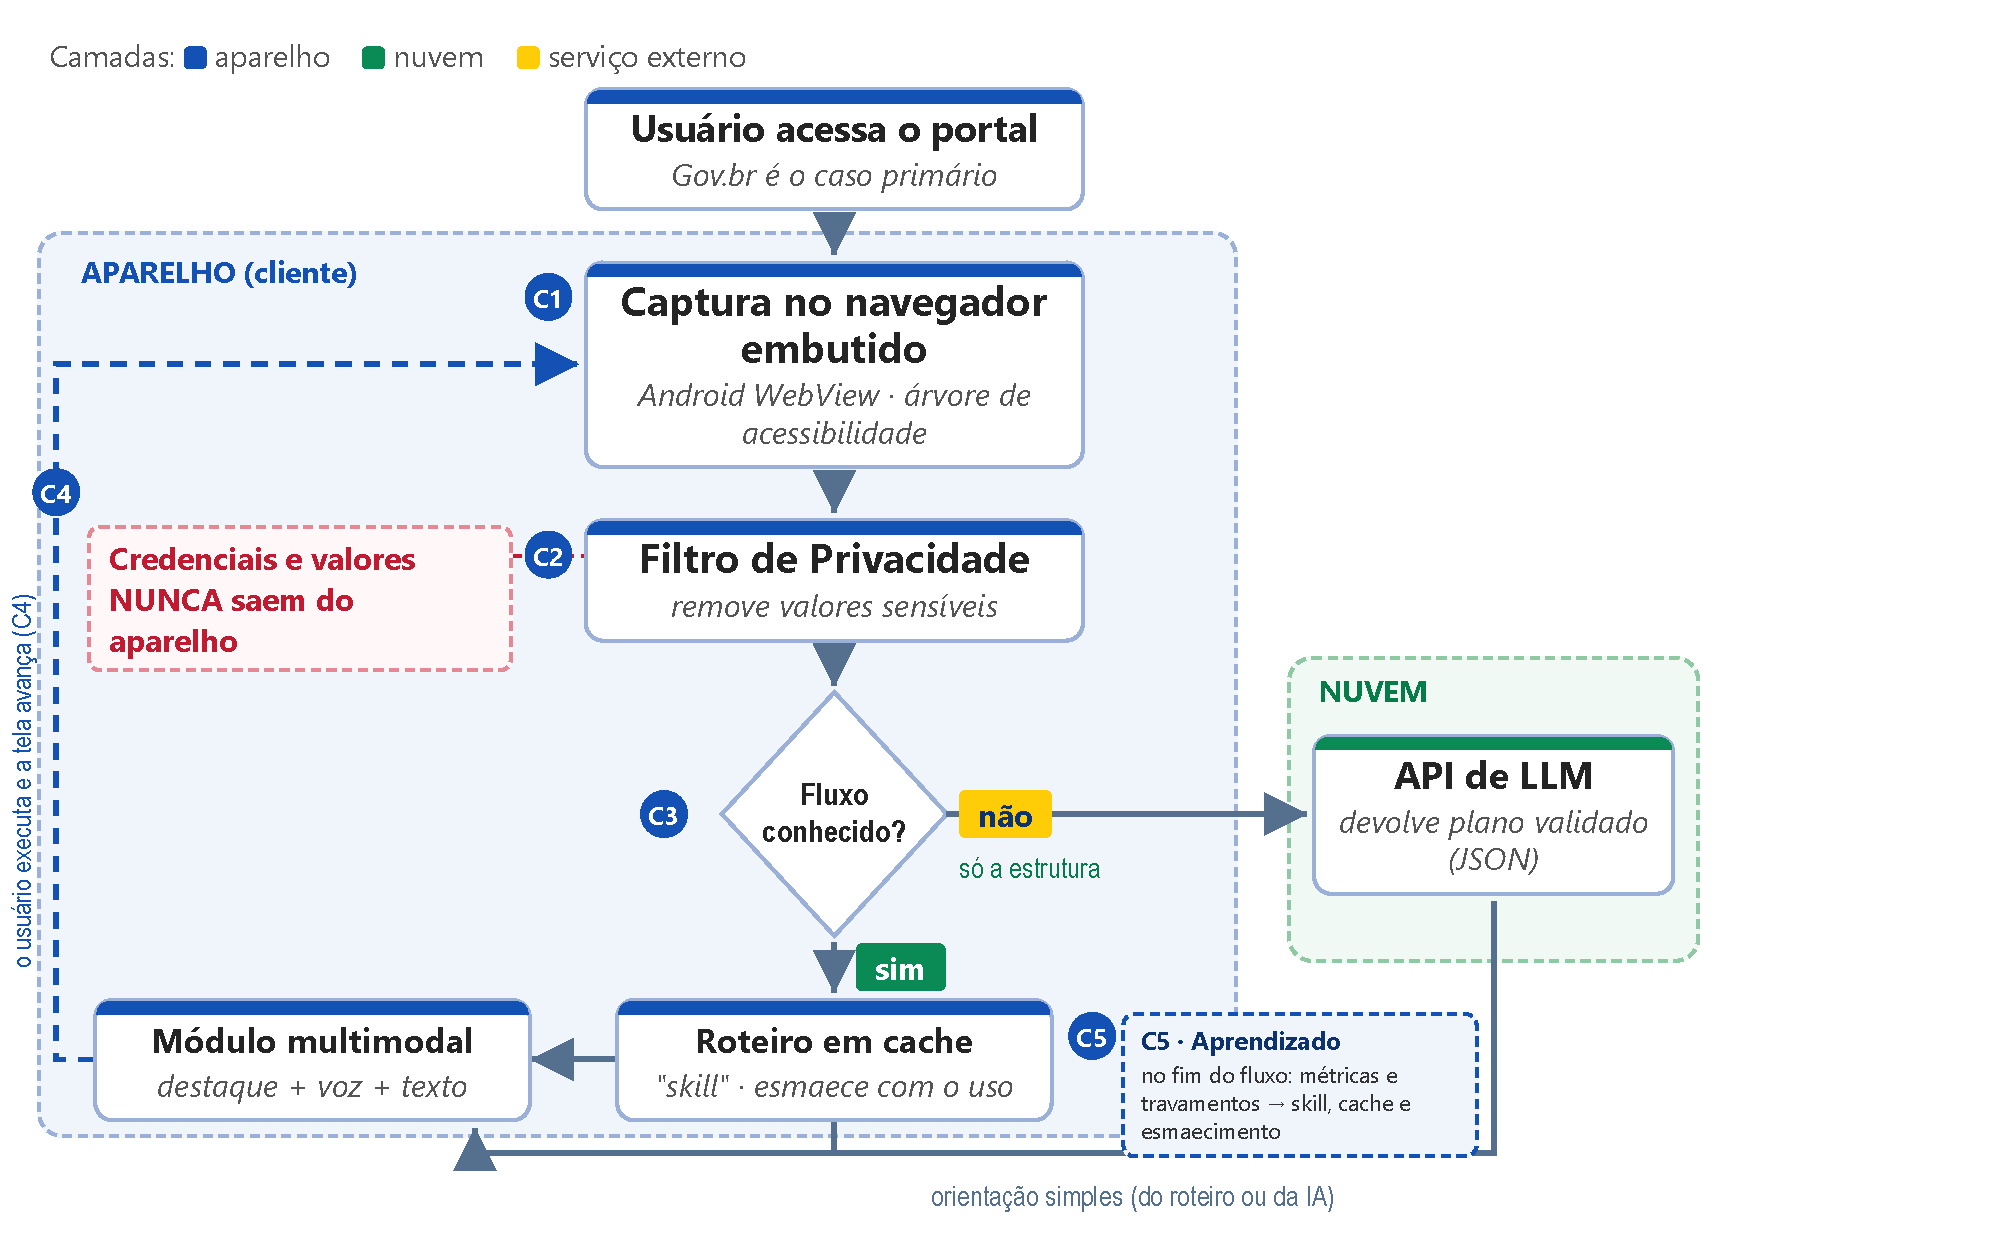
\includegraphics[width=\textwidth]{Figuras/Diagrama_Fluxo_System.pdf}
  \caption{Fluxo de interação do IAssistente Intergeracional: da captura no navegador embutido à orientação multimodal por voz e destaque visual.}
  \label{fig:fluxo}
\end{figure}

A Figura~\ref{fig:arquitetura} detalha as camadas dessa arquitetura: \emph{scripts} leves de injeção em DOM sobre o Android WebView nativo coletam o contexto da tela; um sanitizador local remove credenciais e dados pessoais antes de qualquer tráfego de rede; e a camada de inteligência consulta modelos acessíveis em \emph{tier} gratuito ou processamento local, com a síntese de voz executada integralmente no aparelho.

\begin{figure}[!ht]
  \centering
  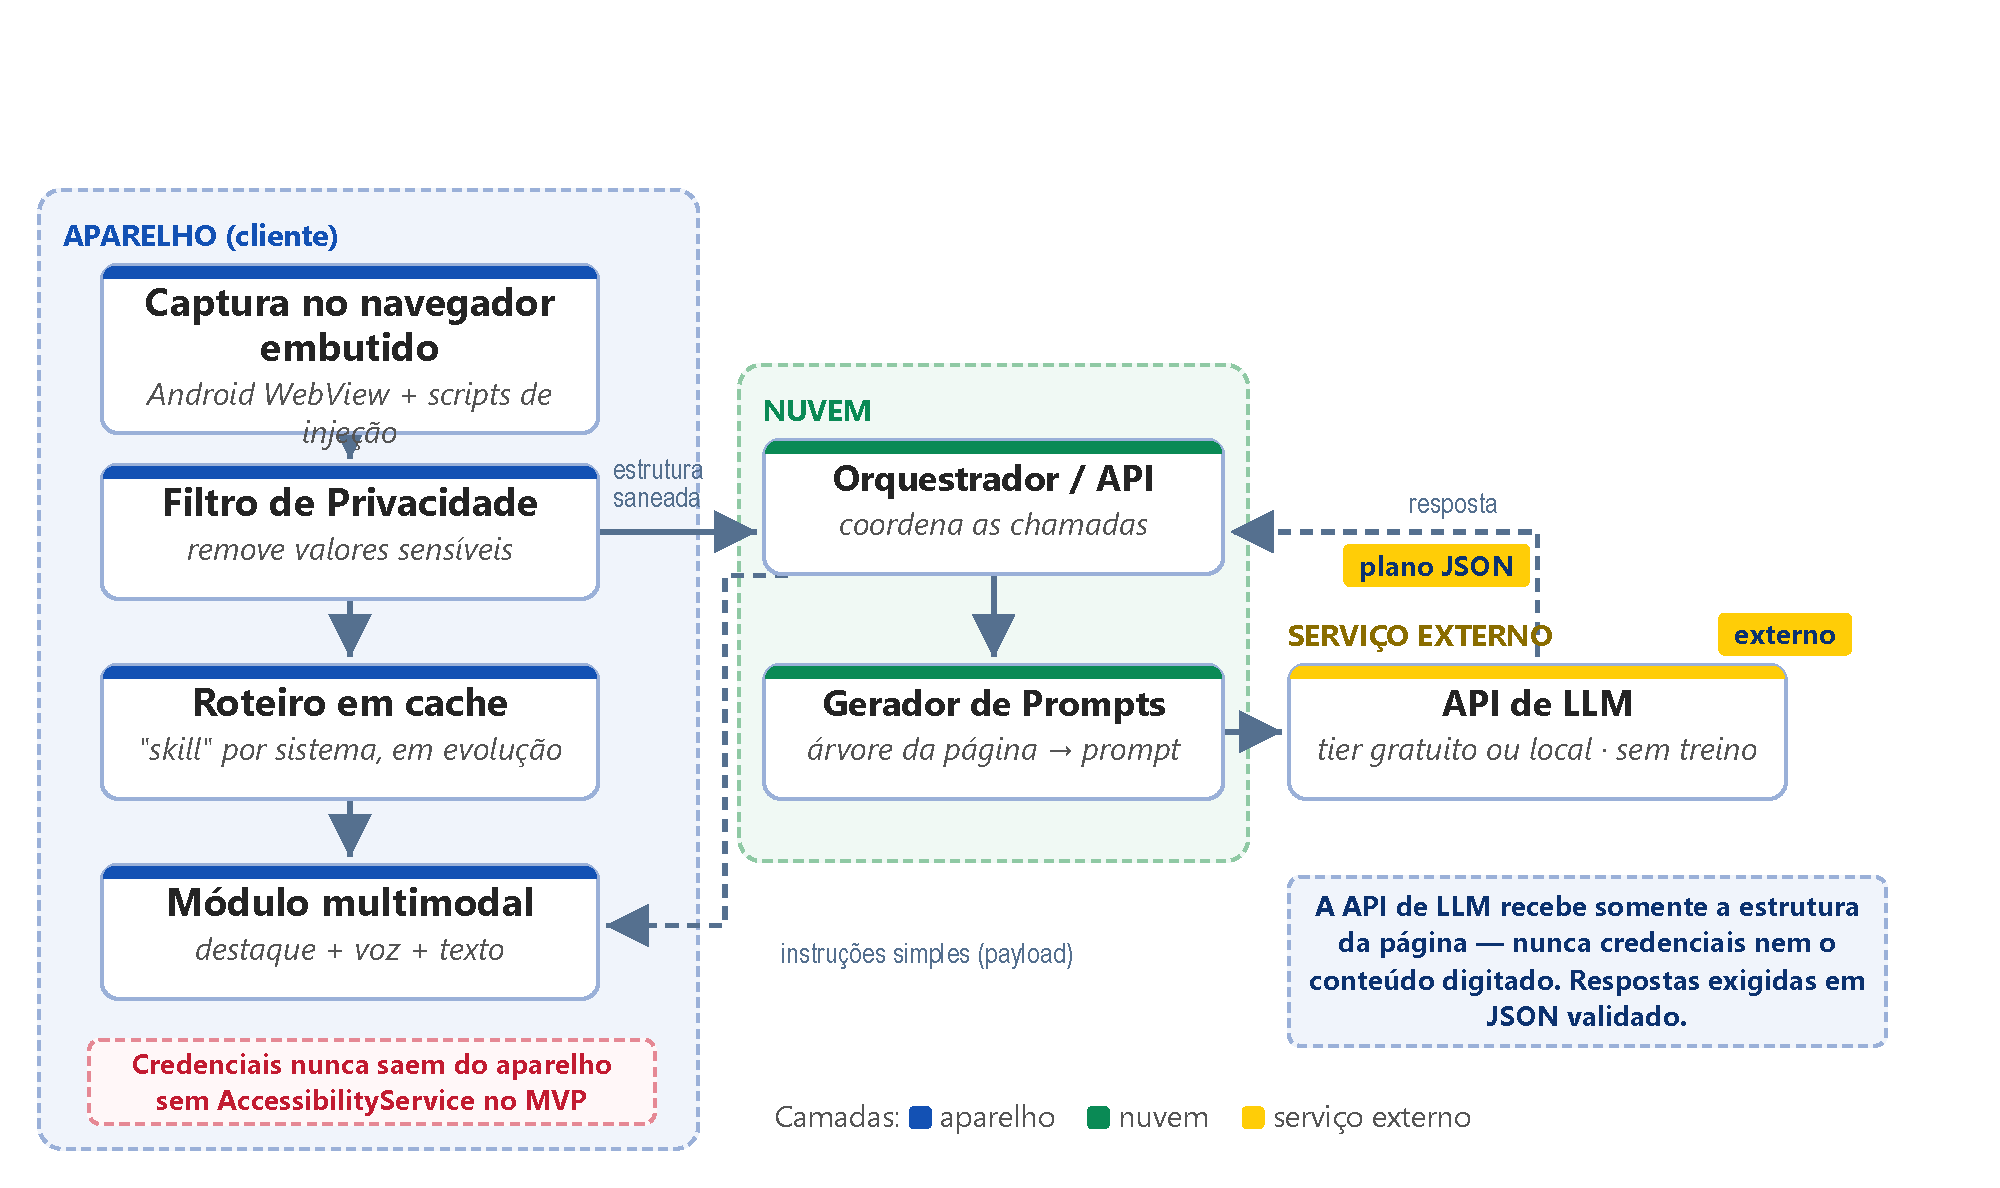
\includegraphics[width=\textwidth]{Figuras/Arquitetura_Detalhada.pdf}
  \caption{Arquitetura em camadas do sistema: captura em DOM sobre o Android WebView nativo, sanitização local de dados e camada de inteligência em \emph{tier} gratuito ou local.}
  \label{fig:arquitetura}
\end{figure}

\subsection{Requisitos Funcionais (RF) e Não Funcionais (RNF)}

\begin{itemize}
  \item \textbf{RF01 -- Captura Semântica:} mapear elementos visuais da página aberta no navegador integrado.
  \item \textbf{RF02 -- Tradução de Erros:} converter mensagens técnicas de erro em linguagem clara e acolhedora.
  \item \textbf{RF03 -- Feedback Multimodal:} exibir destaque visual amarelo/verde nos botões e ditar o passo por voz.
  \item \textbf{RNF01 -- Economia de Dados:} manter roteiros de navegação comuns salvos localmente (\emph{cache}/SQLite).
  \item \textbf{RNF02 -- Privacidade LGPD:} garantir que credenciais e dados pessoais jamais saiam do aparelho.
\end{itemize}

A Figura~\ref{fig:mockup} ilustra a interface principal do aplicativo em uso sobre um serviço público real (Gov.br): o campo a ser preenchido recebe borda de destaque, o passo atual é lido em voz alta, e erros técnicos são traduzidos para uma frase simples e acolhedora.

\begin{figure}[!ht]
  \centering
  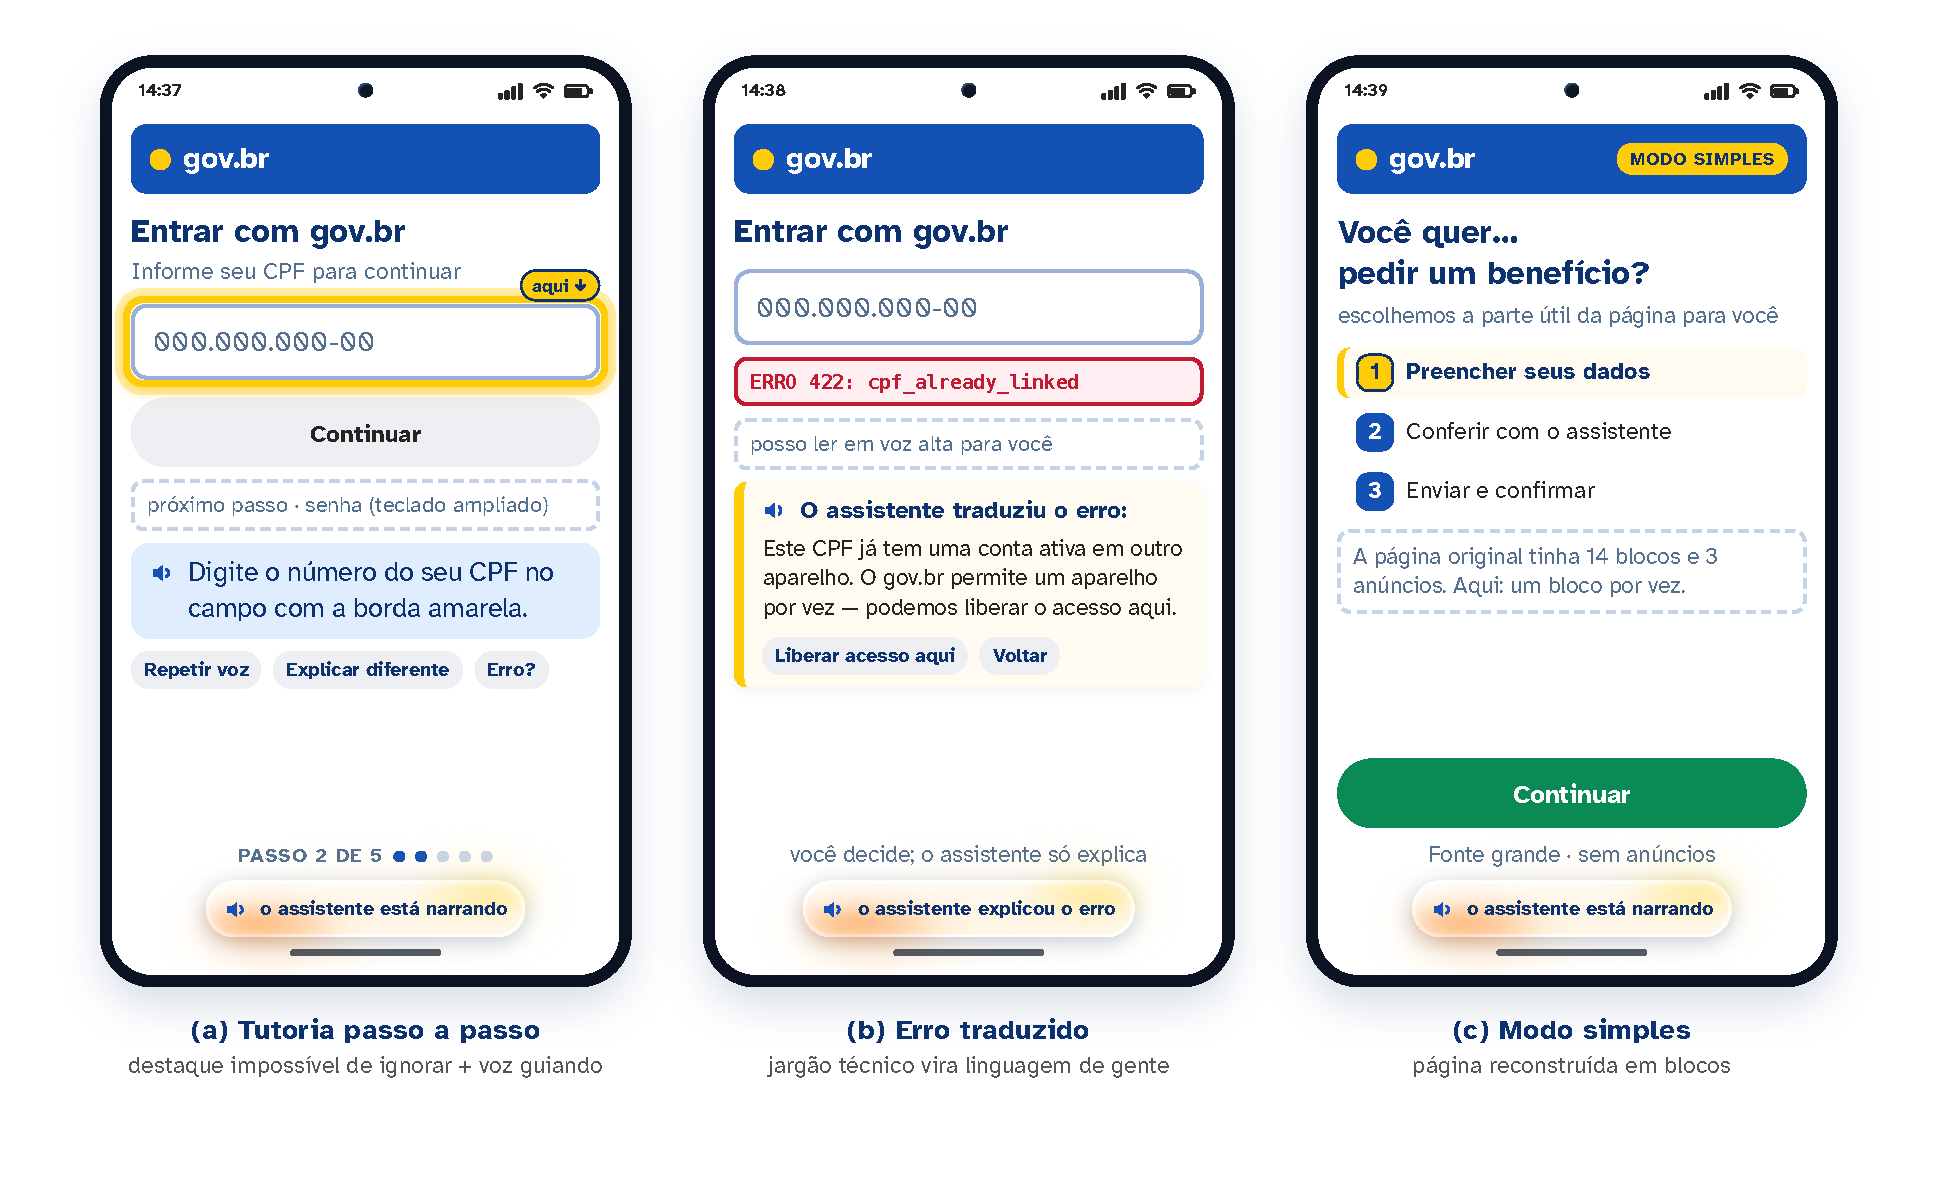
\includegraphics[width=0.92\textwidth]{Figuras/Funcionalidades_Mockup.pdf}
  \caption{Mockup da interface principal: destaque visual no campo ativo, leitura em voz alta do passo atual e tradução de erros para linguagem simples sobre o Gov.br.}
  \label{fig:mockup}
\end{figure}

\section{Conclusão e Trabalhos Futuros}

O Projeto Farol demonstra que é viável aplicar inteligência artificial e acessibilidade em projetos escolares do Ensino Médio sem a necessidade de investimentos financeiros elevados. A arquitetura adaptada viabiliza o aprendizado prático de programação web, \emph{mobile} e IHC por estudantes de baixa renda, enquanto entrega uma solução real de impacto social para idosos e PcDs na região de Bragança-PA.

Como trabalhos futuros, estão previstos os testes práticos de usabilidade com a comunidade local, o refinamento das instruções de voz e a criação de novos roteiros de tutoria para serviços municipais.

\bibliographystyle{sbc}
\bibliography{Referencias/referencias}

\end{document}
